\documentclass{article}[10pt]
\usepackage{titling}
\setlength{\droptitle}{-4em}
\usepackage[margin=1in]{geometry}
\usepackage{amssymb}
\usepackage{epsfig}
\usepackage{subfigure}
\usepackage{graphicx}
\usepackage{wrapfig}
\usepackage{setspace}
\usepackage{textcomp}
\usepackage{cite}
\usepackage{float}
\usepackage{csquotes}
\usepackage{graphicx}
\makeatletter
\makeatother

\expandafter\let\csname equation*\endcsname\relax
\expandafter\let\csname endequation*\endcsname\relax
\usepackage{amsmath}
\newcommand{\agt}{\mathrel{\raise.3ex\hbox{$>$\kern-.75em\lower1ex\hbox{$\sim$}}}}
\begin{document}

\title{\emph{Frankenstein} and the horrors of competitive exclusion}


\author{Nathaniel J. Dominy${}^{1,*}$ \& Justin D. Yeakel${}^2$\\
\small{${}^1$Department of Anthropology, Dartmouth College, New Hampshire, USA;}\\
\small{${}^2$Santa Fe Institute, Santa Fe, New Mexico, USA;}\\
\small{${}^*$Email: nathaniel.j.dominy@dartmouth.edu}}

\date{}
% \begin{abstract}
%
%
% \end{abstract}


\maketitle
\vspace{-1cm}

Bicentennial celebration of the inception of \textit{Frankenstein} invites the present article on Victor Frankenstein and his fateful decision to destroy an unfinished female creature. 
The act itself was impulsive (caused by a `sensation of madness'), but it was preceded with agonized reasoning that would be familiar to any contemporary ecologist or evolutionary biologist. 
Here we present a formal treatment of Frankenstein's reasoning and show that his rationale for denying a mate to his male creation has empirical justification.
It was a prudent decision, averting our own extinction by competitive exclusion. 
Our results suggest that the central horror of Mary Shelley's novel lies in its prescient command of foundational concepts in ecology and evolution.



Some background: Victor Frankenstein created and then disavowed a nameless male creature described as eight feet in height, and proportionally large. 
For three years, the frightened creature wandered the European wilderness, becoming considerate and literate in three languages. 
He then reunites with Frankenstein in Switzerland and pleads for a female companion `of the same species' to mitigate his loneliness. Crucially, and cleverly, the creature appears to anticipate and prempt concerns of direct competition with humans; he promises geographic isolation and emphasizes resource partitioning:


\begin{displayquote}
\emph{If you consent, neither you nor any other human being shall ever see us again: I will go to the vast wilds of South America. My food is not that of man; I do not destroy the lamb and the kid to glut my appetite; acorns and berries afford me sufficient nourishment. My companion will be of the same nature as myself, and will be content with the same fare. We shall make our bed of dried leaves; the sun will shine on us as on man, and will ripen our food.}
\end{displayquote}

Frankenstein concedes and commences work on a female creature. 
However, he soon reflects on the potential for population growth and direct competition: \emph{a race of devils would be propagated upon earth who might make the very existence of the species of man a condition precarious and full of terror.}
The nature of this terror is revealed as he considers the probability of human extinction: \emph{future ages might curse me as their pest, whose selfishness had not hesitated to buy its own peace at the price, perhaps, of the existence of the whole human race.}


Here we indulge this conjecture by asking if and when a population of creatures $C$ could drive a population of humans $H$ to extinction.
We elevated a tacit assumption to a formal parameter \textendash{that the intelligence, resilience, and dietary breadth of creatures confers a competitive advantage\textendash} and used a classic Lotka-Volterra competition framework to determine changes in population trajectories, where the effect of creatures on humans (which is always harmful by direct or indirect competitive interaction) is $a_{HC}$, and the effect of humans on creatures is $a_{CH}$, where $a_{HC} > a_{CH}$ maintains a competitive advantage for creatures.
Given growth rates for humans $r_H$ and creatures $r_C$, as well as a carrying capacity for both $k$, the 2-D continuous time model is written
\vspace{-1mm}
\begin{align}
\dot{H}&=r_H H\left(1 - (H + a_{HC} C)/k\right), \\ \nonumber	
\dot{C}&=r_C C\left(1 - (C + a_{CH} H)/k\right),
\end{align}

\noindent where human extinction is inevitable.
However, the time to extinction could be as much as $t_e=10^8$ years, which is tantamount to species coexistence at biological timescales.

Such an outcome is hardly surprising given that the human population of 1816 would have exceeded a founding population of two creatures by nine orders of magnitude.
The population of Europe was then $178\times 10^6$, whereas the global population was $1.01\times 10^9$ (with an assumed carrying capacity of $k=10^{10}$).
Given a human growth rate (= birth rate - death rate) of $r_H=0.0067$, there is little reason for Frankenstein to envision imminent extinction. 
Yet the creature is known to have recovered from a gunshot wound that `shattered flesh and bone', suggesting that reanimated tissue is resistant to necrosis. 
If undead tissue dies at a slower rate than human tissue, then it follows that creatures would have a correspondingly lower death rate, such that the overall growth rate is $r_C=1.5\times$ that of humans.


These parameters shed new light on Frankenstein's decision to destroy his unfinished female creature.
If we assume direct competition with humans in 1816, and if we allow the competitive advantage of creatures to vary from $\epsilon=2\times$ to $\epsilon=10\times$ that of humans, then we can assess extinction time as a function of competition.
In other words, $a_{HC} = \epsilon a_{CH}$, where the effect of creatures on humans is $\epsilon \times$ the effect of humans on creatures.

\begin{wrapfigure}{r}{0.35\textwidth}
\singlespacing
  \vspace{-35pt}
  \begin{center}
    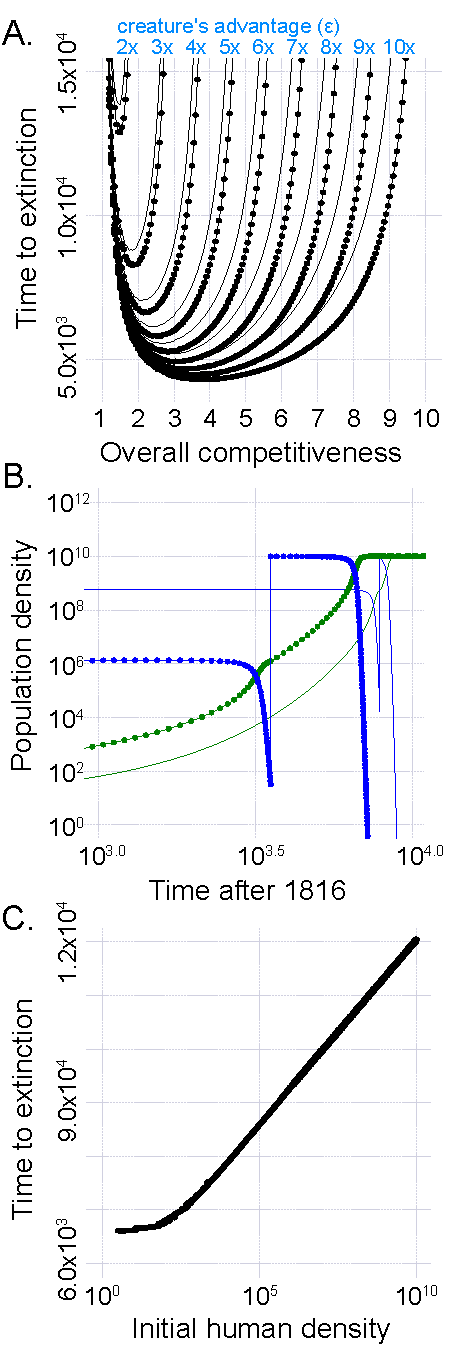
\includegraphics[width=0.3\textwidth]{fig_combined.pdf}
  \end{center}
  \vspace{-10pt}
  \caption{\footnotesize 
  A. Extinction time given competitive environment.
  B. Population trajectories for humans (blue) and creatures (green) given initial growth in the Amazon (dotted) and Europe (solid).
  C. Time to extinction vs. the human population size during initial growth of the creature population.
  }
  \vspace{2pt}
    \label{fig}
\end{wrapfigure}
When competition is low, the time to human extinction is effectively infinite, meaning that creatures and humans can coexist (Fig. 1A).
However, as competition increases, our model shows that the time to human extinction drops precipitously to a minimum and then increases, an effect that becomes more exaggerated as the competitive advantages of creatures increase.
Intriguingly, if the overall level of competition is high, the creatures are doomed to extinction despite their competitive advantage, such that the time to human extinction is also infinite.
This result occurs because the population of creatures begins at $n=2$ individuals, a population size that is too small for establishing a competitive foothold.
In the worst case scenario ($a_{HC}=3.5, \epsilon=10$), our global model indicates human extinction in $t_e = 4188$ years.

Given the large disparity in population sizes, it is worth considering the effects of different environmental parameters at the onset of competitive interactions between creatures and humans.
Recall that the creature promised to inhabit `the vast wilds of South America' in an apparent gesture of conciliation.
We therefore explored the effects of dispersal by comparing competitive interactions of creatures and humans in the Amazon catchement (dotted curves, Fig. 1A,B) and Europe (solid curves, Fig. 1A,B).
We assume that when the population of creatures reaches 90\% of the carrying capacity of either environment, it will begin direct competion with the global human population.

A founding population of two creatures in South America (green dotted line, Fig. 1B) would quickly surpass the local human population (blue dotted line, Fig. 1B -- the vertical jump denotes the transition from regional to global competition) and drive humans to extinction faster than competition in Europe (creatures: green solid line; humans: blue solid line; Figure 1B).
The lower $t_e$ for this scenario holds across all levels of competition and for all values of $\epsilon$ (dotted curves, Fig. 1A).
The wilds of South America would therefore accelerate the population growth of creatures, at least compared to the slower dynamics that would have occurred in Europe with its larger human population.
In general, we find that low-density --and by extension low competition-- initial environments can catalyse the establishment of an invading population, thereby hastening the extinction of a resident population (Fig. 1C).

The present findings are drawn from a work of science fiction but the importance is threefold. 
First, our results reinforce and expand the gothic tone of \textit{Frankenstein} and its underlying exploration of moral and scientific responsibility.
Second, our results cast new light on the creature and his motives for inhabiting the wilds of South America, a lower-competition environment.
Third, our results bolster the speculative concerns of Frankenstein with empirical support -- humans would indeed face species interactions `full of terror'. 
The nature of this terror is termed competitive exclusion, a concept that escaped definition until the early 20th Century. 
We conclude by suggesting that the central horror and genius of Mary Shelley's novel lies in its early mastery of foundational concepts in ecology and evolution.
%Indeed, the creature's concession to escape to the wilds of South America may have been a worst-case scenario, motivating Frankenstein to destroy the creature's companion, and eventually leading to the deaths of those he loved as well as his own.

%In Europe, XXXX years elapse before the creature population (green solid lines, Fig. 1B) overtakes humans (blue solid lines, Fig. 1B), and an additional XXXX years for it to drive humans extinct (we note that humans are assumed to have reached global carrying capacity by the time the creature population can compete globally). 
%If the creatures begins reproducing in the Amazon, XXXX elapse before the Amazon is overtaken, with another XXXX years before the global population of humans are driven extinct.

%The general conclusion -- invading via a catalyst
%We have shown with a simple model that the initial population growth of an invading organism (the creature) within a low-density -- and by extension low-competition -- environment can catalyze the invader's success, lowering the timescale of invasion to the exclusion of a resident species (humans).
%Many invading species in ecological systems have competitive advantages over residents such that even small competitive effects on the resident can lead to extinction over ecological timescales, and this also holds for Frankenstein's potential derivation of creature population growth (Fig. 1A).
%The decision that Frankenstein makes, at the cost of his own destruction, was thus prescient, demonstrating that Shelley had an implicit understanding of the dynamics and potential horrors of niche overlap and competitive exclusion of invading species.
%These issues are pertinent to our own world, which is now replete with \emph{creatures}:
%species left to invade after native environments are destroyed or fragmented,
%species that are distributed across the world by global transportation networks,
%and species that are created or modified to suite our own needs.
%In the bicentennial of Mary Shelley's Frankenstein, perhaps there is no better time to reconsider Frankenstein's creation and the horrors of competitive exclusion.




\end{document}














